\documentclass[conference, 10pt, twocolumn]{ieeeconf}

\IEEEoverridecommandlockouts
\overrideIEEEmargins


\usepackage[usenames]{color}
\usepackage{enumerate}
\usepackage{url}
\usepackage{subfigure}
\usepackage{amsfonts,mathrsfs}
\usepackage{amssymb,amsmath}
\usepackage{verbatim}
\usepackage{acronym}
\usepackage{mathtools}
\usepackage{graphicx}
\usepackage{bbm}

%\newcommand{\remove}[1]{}
%\def\jnt#1{{{\bf #1}}}
\def\rasoul#1{{\color{blue}#1}}
%\long\def\red#1{{{\color{red}#1}}}
\def\an#1{{{\bf \color{red}#1}}}
\def\fskip#1{}

\newcounter{note}
\newtheorem{theorem}{Theorem}
\newtheorem{assumption}{Assumption}
\newtheorem{algorithm}[theorem]{Algorithm}
\newtheorem{axiom}[theorem]{Axiom}
\newtheorem{case}[theorem]{Case}
\newtheorem{claim}[theorem]{Claim}
\newtheorem{conclusion}[theorem]{Conclusion}
\newtheorem{condition}[theorem]{Condition}
\newtheorem{conjecture}[theorem]{Conjecture}
\newtheorem{corollary}{Corollary}
\newtheorem{criterion}[theorem]{Criterion}
\newtheorem{definition}{Definition}
\newtheorem{example}{Example}
\newtheorem{exercise}[theorem]{Exercise}
\newtheorem{lemma}{Lemma}
\newtheorem{notation}[note]{Notation}
\newtheorem{problem}[theorem]{Problem}
\newtheorem{proposition}[theorem]{Proposition}
\newtheorem{remark}{Remark}
\newtheorem{solution}[theorem]{Solution}
\newtheorem{summary}[theorem]{Summary}
\newtheorem{acknowledgement}{Acknowledgement}


%\textwidth 6.2in \textheight 9in \setlength{\topmargin}{-0.3in}
%\setlength{\oddsidemargin}{0.1in} \setlength{\evensidemargin}{0.1in}
%\renewcommand{\theequation}{\thesection.\arabic{equation}}
\renewcommand{\theenumi}{\arabic{enumi}}
\newcommand{\qed}{\ \ {\bf q.e.d.}}

\def\1{{\bf 1}}
\def\al{\alpha}
\def\E{\mathcal{E}}
\def\Eb{\overline{\E}}
\def\L{\mathcal{L}}
\def\A{\mathcal{A}}
\def\Ps{P_{\sigma}}
\def\e{{\bf e}}
\def\ei{{\e^{(i)}}}
\def\ej{{\e^{(j)}}}
\def\ek{{\e^{(k)}}}
\def\B{{\mathcal B}}
\def\Pm{{\mathcal P}}
\def\Gb{\overline{G}}
\def\N{\mathbb{N}}
\def\F{\mathscr{F}}
\def\Finf{\mathscr{F}^{\infty}}


\def\ol{\bar}
\def\Rd{\mathbb{R}^d}
\def\l{\lambda}
\def\b{\beta}
\def\d{\delta}
\def\e{\epsilon}
\def\g{\gamma}
\def\a{\alpha}
\def\N{\mathcal{N}}
\def\s{\sigma}
\def\tl{\tilde}
\def\k{\kappa}
\def\o{\omega}
\def\rn{\mathbb{R}^n}

\def\R{\mathbb{R}}
\def\re{\mathbb{R}}
\def\gr{\nabla}
\def\cone{{\rm cone}}
\def\dist{{\rm dist}}
\def\t{\tau}
\def\qed{\ {\bf Q.E.D.}}
\def\S{\mathscr{S}}
\def\bS{\mathbb{S}}
\def\cS{\mathcal{S}}
\def\I{\mathscr{I}}
\def\Z{\mathbb{Z}}

\newcommand{\EXP}[1]{\mathsf{E}\!\left[#1\right] }
\newcommand{\prob}[1]{\mathsf{Pr}\left( #1 \right)}
\newcommand{\remove}[1]{}
\newcommand{\Rm}{\mathbb{R}^m}
\newcommand{\lra}{\leftrightarrow}
\newcommand{\lrA}{\Leftrightarrow}
\newcommand{\M}{\mathscr{M}_2}
\newcommand{\diag}{\mbox{diag}}
\newcommand{\Ginf}{G^{\infty}}
\newcommand{\Einf}{\mathscr{E}^{\inf}}
\newcommand{\tw}{\tilde{W}}
\newcommand{\xc}{\{x(k)\}}
\DeclarePairedDelimiter\ceil{\lceil}{\rceil}
\DeclarePairedDelimiter\floor{\lfloor}{\rfloor}

\newcommand{\todo}[1]{\vspace{5 mm}\par \noindent \marginpar{\textsc{ToDo}}
\framebox{\begin{minipage}[c]{0.9 \columnwidth} \tt #1
\end{minipage}}\vspace{5 mm}\par}

\def\argmin{\mathop{\rm argmin}}
\def\an #1{{\color{red} #1}}

\begin{document}
\title{Random Tree Search Algorithm for Nash Equilibrium in Capacitated Selfish
Replication Games}
\author{\authorblockN{Seyed Nematollah Ahmadian\textdagger, Seyed Rasoul Etesami\textdaggerdbl, H. Vincent Poor\textdaggerdbl}
  \authorblockA{}
\thanks{\textdagger Seyed Nematollah Ahmadian is with
Coordinated Science Laboratory,
Department of Electrical and Computer Engineering,
University of Illinois at Urbana-Champaign, Urbana, IL, 61801;
E-mail: {ahmadya2}@illinois.edu}
\thanks{
\textdaggerdbl Seyed Rasoul Etesami and H. Vincent Poor are with
Department of Electrical Engineering,
Princeton University, NJ, 08644;
E-mail: etesami,poor@Princeton.EDU}
}
\maketitle
\begin{abstract}
In this paper we consider a resource allocation
game with limited capacities over large scale networks and
propose a novel randomized algorithm for searching its purestrategy
Nash equilibrium points. It is known that such games
always admit a pure-strategy Nash equilibrium and benefit
from having a low price of anarchy. However, the best
theoretical results only provide a quasi-polynomial constant
approximation algorithm of the equilibrium points over general
networks. Here, we search the state space of the resource
allocation game for its equilibrium points. We use a random
tree based search methods to minimize a proper objective
function and direct the search toward the pure-strategy Nash
equilibrium points of the system. Through empirical results, we
demonstrate that in comparison to the best known theoretical
bounds, our technique is more efficient.
\end{abstract}
\begin{keywords}
Capacitated selfish replication game; pure Nash equilibrium (NE); Random tree algorithm.
\end{keywords}

\section{Introduction}
In recent years, there has been a wide range of studies on the role of social and distributed networks in various disciplinary areas such as economics, computer science, epidemiology, and engineering. In particular, availability of large data from online social networks and advances in control of distributed systems have drawn the attention of many researchers to model various phenomena in social and distributed networks using some mathematical tools such as game theory in order to exploit some of the hidden properties of such networks. Such studies not only improve our understanding of the complex nature of social and distributed events, but also enable us to devise more efficient algorithms toward some desired outcomes in such networks. 

Due to accelerated growth of economic networks and advances in using game-theoretic tools in various applications, modeling of distributed network storage has become an important issue. In general, distributed network storage games or resource allocation games are characterized by a set of agents who compete for the same set of resources \cite{pacifici2012convergence,masucci2014strategic}, and arise in a wide variety of contexts such as congestion games \cite{milchtaich1996congestion,ackermann2008impact,fabrikant2004complexity}, load balancing \cite{ghosh1994dynamic}, peer-to-peer systems \cite{pollatos2008social}, web-caches \cite{gopalakrishnan2012cache}, content management \cite{pollatos2008social}, and market sharing games \cite{goemans2006market}. Among many problems that arise in such a context, one that stands out is distributed replication, which not only improves the availability of resources for users, but also increases the reliability of the entire network with respect to customer requests \cite{chun2004selfish}, \cite{goyal2000learning}.           

Distributed replication games with servers that have access to all the resources and are accessible at some cost by users have been studied in \cite{laoutaris2006distributed}. Moreover, the uncapacitated selfish replication game where the agents have access to the set of all resources was studied in \cite{chun2004selfish}, where the authors were able to characterize the set of equilibrium points based on the parameters of the problem. However, unlike the uncapacitated case, there is no comparable characterization of equilibrium points in capacitated selfish replication games. In fact, when the agents have limited capacity, the situation could be much more complicated as the constraint couples the actions of agents much more than in the uncapacitated case or in replication games with servers. 

Typically, capacitated selfish replication games are defined in terms of a set of available resources for each player, where the players are allowed to communicate through an undirected communication graph. Such a communication graph identifies the access cost among the players, and the goal for each player is to satisfy his/her customers' needs with minimum cost. Ideally, and in order to avoid any additional cost, each player only wants to use his/her own set of resources. However, due to limitation on capacity, players do not have access to all the resources and hence, they incur some cost by traveling over the network and borrowing some of the resources which are not available in their own caches from others in order to meet their customers' demands. The problem of finding an equilibrium for capacitated selfish replication games in the case of hierarchical networks was studied in \cite{gopalakrishnan2012cache}. Moreover, the class of capacitated selfish replication games with binary preferences has been studied in \cite{gopalakrishnan2012cache,etesami2014pure}, where ``binary preferences" captures the behavioral pattern where players are
equally interested in some objects. 

In this paper, we consider the capacitated selfish replication game with binary preferences. In this model players act myopically and selfishly, while they are required to fully satisfy their customers' needs. Note that, although the players act in a selfish manner with respect to others in satisfying their customer needs, their actions are closely coupled with the others' and they do not have absolute freedom in the selection of their actions. It was shown in \cite{gopalakrishnan2012cache} that when the number of resources is 2, there exists a polynomial time algorithm $\mathcal{O}(n^3)$ to find an equilibrium. This result has been improved in \cite{etesami2014pure} to a linear time algorithm when the number of resources is bounded above by 5. However, in general there exist only exponential time algorithms for finding a pure-strategy Nash equilibrium. In this work we consider such games over general undirected networks and devise randomize algorithm based on random tree search to find the Nash equilibrium points of the system.
 
The paper is organized as follows. In Section~\ref{sec:game-model}, we introduce capacitated selfish replication games with binary preferences over general undirected networks. We review some salient properties of such games and include some relevant existing results on this problem. In Section \ref{sec:main-I}, we provide we characterzie the equilibrium points of the system as maximizers of a well-defined function and theroreticaly justify that randomization can be very beneficial for maximizing such function under certain cases. Following this, in Section \ref{sec:apx-alg} we device a random tree search algorithm for maximize the objective function and through numerous simulations we show that this method can be quite effective. We conclude the paper with identifying future directions of research in Section~\ref{sec:conclusion}. 

\textbf{Notations}: 
For a positive integer $n$, we let $[n]:=\{1,2,\ldots,n\}$. For a vector $v\in \R^n$, we let $v_i$ be the $i$th entry of $v$. We use $\mathcal{G}=([n], \mathcal{E})$ for an undirected underlying network with a node set $\{1,2,\ldots,n\}$ and an edge set $\mathcal{E}$. For any two nodes $i, j \in [n]$, we let $d_{\mathcal{G}}(i,j)$ be the graphical distance between them, that is, the length of a shortest path which connects $i$ and $j$. The diameter of a graph, denoted by $D$, is the maximum distance between any pair of vertices, that is, $D=\max_{i,j \in [n]} d_{\mathcal{G}}(i,j)$. Moreover, for an arbitrary node $i\in [n]$ and an integer $r\ge 0$, we define a ball of radius $r$ and center $i$ to be the set of all the nodes in the graph $\mathcal{G}$ whose graphical distance to the node $i$ is at most $r$, i.e., $B(i,r)=\{x\in \mathcal{V}| d_{\mathcal{G}}(i,x)\leq r\}$. We denote a specific Nash equilibrium by $P^*$. Finally, we use $|S|$ to denote the cardinality of a finite set $S$.
 
\section{Problem Formulation and Existing Results}\label{sec:game-model}

In this section we first introduce the capacitated selfish replication game with binary preferences as was introduced in \cite{gopalakrishnan2012cache}. In the balance of this paper, our focus will be on such games, which for simplicity we refer to as CSR games.

\subsection{CSR Game Model}
We start with a set of $[n]=\{1,2,\ldots,n\}$ nodes (players) which are connected by an undirected graph $\mathcal{G}=([n], \mathcal{E})$. We denote the set of all resources by $O=\{o_1, o_2,\ldots, o_k\}$. For simplicity, but without much loss of generality, we assume that each node can hold only one resource in its cache. All the results can in fact be extended to CSR games with different capacities (see Remark \ref{rem:varying-cache} below). Moreover, we assume that each node has access to all the resources. For a particular allocation $P=(P_1, P_2, \ldots, P_n)$, we define the sum cost function $C_i(P)$ of the $i$th player as follows:
\begin{align}\label{eq:CSR-cost-formulation}
C_i(P)=\sum_{o\in O\setminus \{P_i\}}d_{\mathcal{G}}(i, \sigma_i(P,o)), 
\end{align}
where $\sigma_i(P,o)$ is $i$'s nearest node holding $o$ in $P$. Given an allocation profile $P$ we define the {\bf\textit{radius}} of agent $i$, denoted by $r_i(P)$, to be the distance between node $i$ and the nearest node other than her holding the same resource as $i$, i.e., $r_i(P)=\min_{ j\neq i, P_j=P_i}d_{\mathcal{G}}(i,j)$. Note that if there does not exist such a node, we simply define $r_i(P)=D$, where $D$ is the diameter of the network. We suppress the dependence of $r_i(P)$ on $P$ whenever there is no ambiguity. In Figure \ref{fig:example-model} we have illustrated an instance of the CSR game for $n=11$ and $|O|=3$, and provided the associated costs and radii for two players $i=1,8$.

\begin{figure}[htb]
\vspace{-1.5cm}
\begin{center}
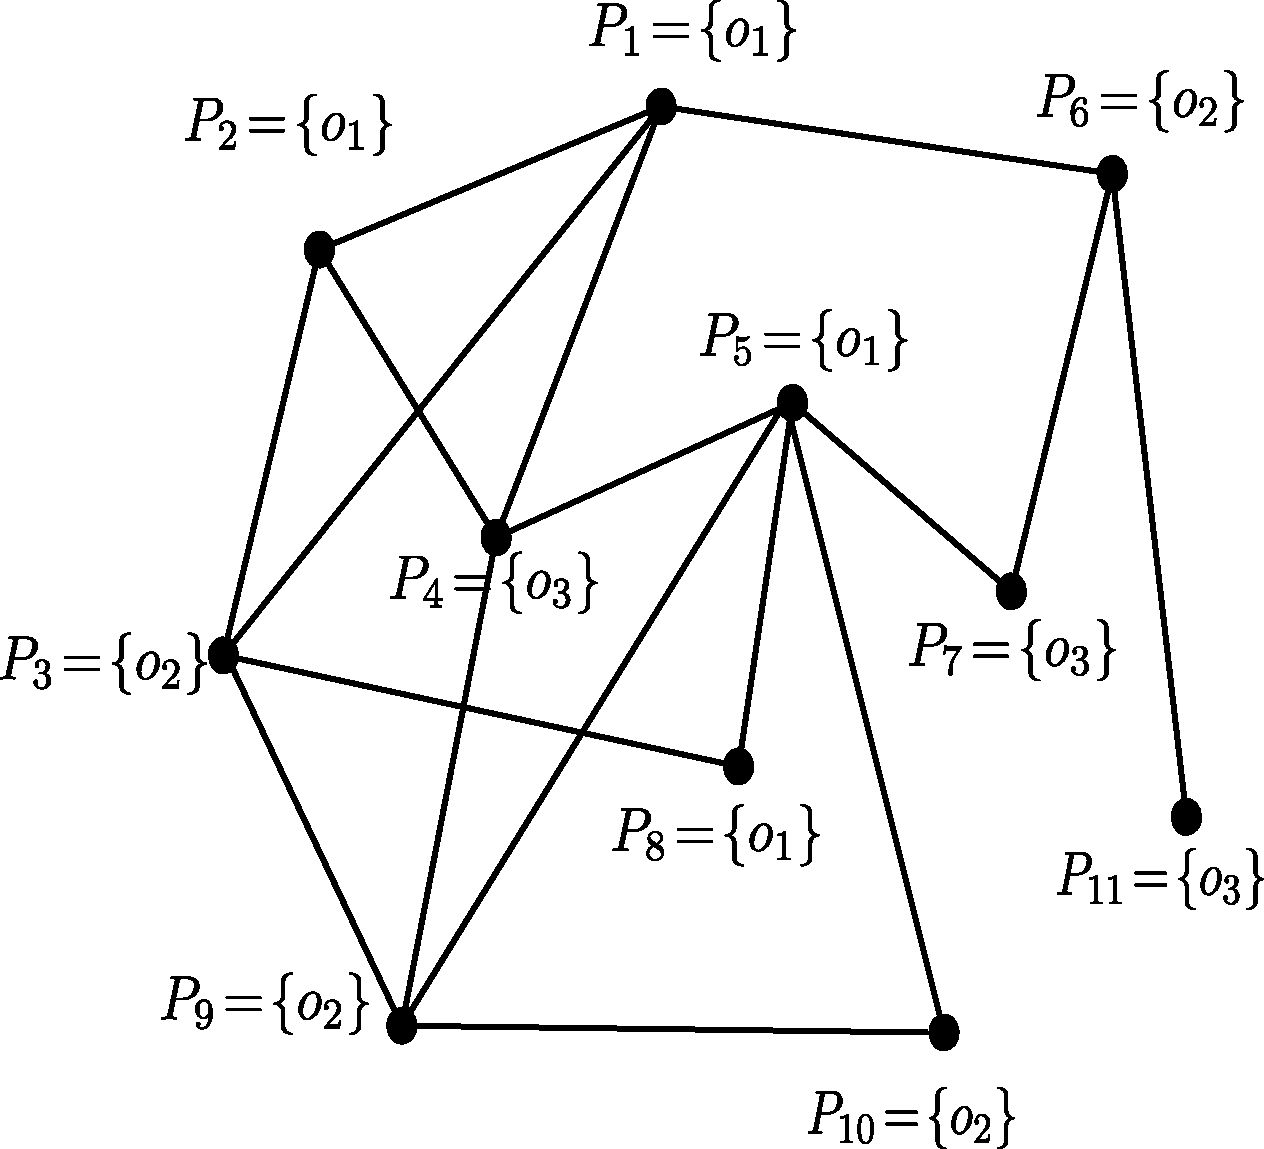
\includegraphics[totalheight=.22\textheight,
width=.4\textwidth,viewport=-50 0 800 750]{example} \hspace{0.4in}
\end{center}
\vspace{-0.3cm}\caption{CSR game with $n=11$ players and $O=\{o_1,o_2,o_3\}$ resources. We have $C_1(P)=0+1+1=2, C_8(P)=0+1+2=3$ and $r_1(P)=1, r_8(P)=1$.}
\label{fig:example-model}
\end{figure}
\vspace{-0.3cm}
\begin{remark}
If some resource $o$ is missing in an allocation profile $P$, we define the cost of each player for that specific resource to be large, e.g., $d_{\mathcal{G}}(i, \sigma_i(P, o)) = D + 1, \forall i \in [n]$. Therefore, for $n \ge |O|$, this incentivizes at least one of the players to allocate the missing resources in the network. In the case where $n < |O|$, all the players will allocate different resources and the game becomes trivial, hence we can simply assume that $n \ge |O|$. 
\end{remark}

\begin{remark}\label{rem:varying-cache}
Actually all the proofs in this paper can be carried over to games with varying capacities by constructing a new network which transfers games with different cache sizes to one with unit size caches \cite{etesami2014pure,gopalakrishnan2012cache}.
\end{remark}

\begin{remark}\label{rem:cost-to-radius}
Given two allocation profiles $P$ and $\tilde{P}$ which only differ in the $i$th coordinate, using \eqref{eq:CSR-cost-formulation} and the definition of the radius, one can easily see that $C_i(P)-C_i(\tilde{P})=r_i(\tilde{P})-r_i(P)$. This establishes an equivalence between decrease in cost and increase in radius for player $i$, when the actions of the other players are fixed. 
\end{remark}

It has been shown in \cite{gopalakrishnan2012cache} that the CSR game has an associated ordinal potential function, and hence, it has at least one pure Nash equilibrium. More precisely

\smallskip
\begin{theorem}\label{thm:existence-NE}
The CSR game admits an ordinal potential function, and hence, a pure-strategy Nash equilibrium.
\end{theorem}

Although Theorem \ref{thm:existence-NE} proves the existence of NE, however, in general it can only gurantee an exponential number of iterations for finding such equilibrium points ($\mathcal{O}(|O|^n)$). Therefore, the main challenge here is to find an efficient way to arrive at an equilibrium which we will address in the remaining of this paper.

\section{Characterization of NE v.s Randomization}\label{sec:main-I}

In this section we first characterize the equilibrium points of the CSR game as maximizers of a proper function. Although this function is not monotone along the trajectories of the best response dynamics, however, it is very useful in a sense that it can improve at most linearly many steps because it admits at most linearly many discrete values. The explicit form of this function and some of its properties has been given in the following lemma: 

\smallskip
\begin{lemma}\label{lem:NE-characterization}
Let $r_i$ be the radius of agent $i$ in an allocation profile $P$, and define $M_i(P)$ to be number of different resources in $B_{\mathcal{G}}(i,r_i)$. Then the function $f(\cdot):\mathcal{P}\rightarrow \mathbbm{R}$ defined by $f(P)=\sum_{i=1}^{n}M_i(P)$ achieves its maximum if and only if $P$ is an equilibrium of the CSR game. 
\end{lemma} 
\begin{proof}
For an arbitrary equilibrium $P^*$ and a specific node $i$ with equilibrium radius $r^*_i$, i.e., $r^*_i=d_{\mathcal{G}}(i,\sigma_i(P^*,P^*_i))$, we note that all the resources must appear at least once in $B_{\mathcal{G}}(i,r^*_i)$. In fact, if a specific resource is missing in $B_{\mathcal{G}}(i,r^*_i)$, then node $i$ can increase its radius by updating its current resource to that specific resource, thereby decreasing its cost (Remark \ref{rem:cost-to-radius}). But this is in contradiction with $P^*$ being an equilibrium. Therefore, for every player $i$ all the resources must appear at least once in $B_{\mathcal{G}}(i,r_i)$, and hence $M_i(P^*)=|O|, \forall i\in [n]$. Therefore, $f(P^*)=n|O|$, which is the maximum possible value that could be taken by $f(\cdot)$ (note that in general we have  $M_i(\cdot)\leq |O|, \forall i$). On the other hand, by Theorem \ref{thm:existence-NE} we know that the CSR game always admits a pure NE, and thus $\max_{P\in \mathcal{P}}f(P)=n|O|$. Therefore, if for some allocation profile we have $f(P)=n|O|$, this implies that $M_i(P)=|O|, \forall i\in [n]$, i.e., for every $i\in [n]$, all the resources appear at least once in $B_{\mathcal{G}}(i,r_i)$, which means that $P$ must be an equilibrium since no agent can increase its radius even further.  
\end{proof}

\smallskip
Using Lemma \ref{lem:NE-characterization}, the problem of finding NE of the system reduces to finding the maximizers of the function $f(\cdot)$. In other words, if we have an efficient algorithm which can find the global maximum of $f(\cdot)$, then we will be able to find the equilibrium points of the system efficiently. Note that here $f(\cdot)$ is not a potential function of the game, however, it can be used to drive the search process to an equilibrium. In the following theorem we show that randomization can be quite useful for maximizing such function when the players' neighborhoods are not saturated with many resources. 

\smallskip
\begin{theorem}\label{thm:randomization}
Given a profile of resources at time $t$, as long as the neighborhood of players are not saturated by more than $\sqrt{|O|}$ resources, i.e., $M_i(t)\leq \sqrt{|O|}, \forall i$, then there exists a resource such that if a player $i$ updates to that specific resource, the value of function $f$ strictly increases.
\end{theorem}
\begin{proof}  
Let us consider an arbitrary player $i$ such that $M_i(t)\leq \sqrt{|O|}$, and let him uniformly and independently update to one of the possible $|O|$ resources, each with probability $\frac{1}{|O|}$. We compute the expected amount of $\mathbb{E}[f(t+1)]$. For this purpose we first consider the expected change in $\mathbb{E}[M_i(t+1)]$:  
\begin{align}\nonumber
\mathbb{E}[M_i(t+1)]&\ge \frac{M_i(t)}{|O|}+\frac{M_i(t)-1}{|O|}\times 1\cr 
&\qquad+\frac{|O|-M_i(t)}{|O|}\times (M_i(t)+1),
\end{align}
where the first term in the above expression is the probability that the resource at time $t+1$ remains the same as that at time $t$, the second term is a lower bound for the case where the resource at time $t+1$ changes to one of the different $M_i(t)-1$ resources in $B(i,r_i(t))$, and finally the last term is a lower bound for the case where the resource at node $i$ changes uniformly to one of the possible $|O|-M_i(t)$ which did not appear in $B(i,r_i(t))$.

Next for any other node $j$ such that $i\in B(j, r_j(t)), j\neq i$ we can write
\begin{align}\nonumber
\mathbb{E}[M_j(t+1)]&\ge \frac{1}{|O|}\times 1+\frac{M_j(t)-1}{|O|}\times M_j(t)\cr 
&\qquad+\frac{|O|-M_j(t)}{|O|}\times (M_j(t)+1),
\end{align}
where the first term is a lower bound for the case where node $i$ attains exactly the same resource as node $i$ in the next time step, the second term upper bounds the case where node $i$ updates to one of the possible $M_j(t)-1$ other than $P_j(t)$ which appeared in $B(j, r_j(t))$, and the last term lower bounds the case where node $i$ changes to one of the possible $|O|-M_j(t)$ which did not appear in $B(j, r_j(t))$. Note that for any other node $j$ which is not included in the above two cases we have $M_j(t+1)=M_j(t)$ (since they are not influenced by the random assignment of player $i$). Therefore, we can write
\begin{align}\nonumber
&\mathbb{E}[f(t+1)-f(t)]=\mathbb{E}[M_i(t+1)-M_i(t)]\cr 
&\qquad\qquad\qquad+\!\!\!\!\!\sum_{j: i\in B(j, r_j(t))}\!\!\!\!\!\mathbb{E}[M_j(t+1)-M_j(t)]\cr 
&\qquad\ge 1-\left(\frac{M_i^2+1-M_i}{|O|}\right)+\!\!\!\!\!\sum_{j: i\in B(j, r_j(t))}\!\!\!\!\!\left(\frac{|O|+1-2M_j(t)}{|O|}\right)\cr 
&\qquad\ge 1-\left(\frac{M_i^2+1-M_i}{|O|}\right) >0,
\end{align}
where the last two inequalities is due to the fact that $M_i(t)\leq \sqrt{|O|}, \forall i$. Therefore, we have shown that $\mathbbm{E}[f(t+1)-f(t)]>0$ which implies that there exists a resource $o$ such that player $i$ can update to it and strictly improve the value of the function $f(\cdot)$. In fact, such a choice of resource can be exhaustively found by trying all the possible $|O|$ resources for node $i$, which takes at most $n|O|^{\frac{3}{2}}$ iterations until the algorithm finds a profile of resources whose objective function $f$ is at least $n\sqrt{|O|}$.
\end{proof}

In fact, Theorem \ref{thm:randomization} guarantees a good improvement in the value of the objective function $f$ as long as there are not too many resources around each player. However, when the system gets closer to its equilibrium points, the speed of progress can be much slower, or there may exist a possibility where the objective function gets stuck in one of its local maximums. To circumvent this issue, we introduce a random tree based search algorithm such that with non vanishing probability the algorithm can always escape from the local maximums, and hence steer the search toward global maximum of the objective function.  


\section{Random Tree Search Algorithm for Finding NE}\label{sec:apx-alg}


\section{Conclusion}\label{sec:conclusion}
In this paper, we have studied the binary-preference capacitated selfish replication (CSR) game over general networks. We have characterized the equilibrium points of the system using a proper objective function. We leveraged this objective function and proposed a randomized algorithm based on the random tree search to find the global maximizers of this function, and hence, the NE points of the system. As an avenue for future research, one possibility is to study the dynamic version of the $CSR$ game, in the spirit of what has been discussed in \cite{fabrikant2003network}.

\bibliographystyle{IEEEtran}
\bibliography{thesisrefs}
\end{document}
